%%%%%%%%%%%%%%%%%%%%%%%%%%%%%%%%%%%%%%%%%%%%%%%%%%%%%%%%%%%%%%%%%
\documentclass[12pt, a4paper, notitlepage, onecolumn]{article}
\usepackage[UKenglish]{babel}                   % UK style
\usepackage[utf8]{inputenc}
\usepackage[margin=1in]{geometry}               % Margin size
\usepackage{hyperref}                           % Coloured hyperlinks
  \hypersetup{colorlinks = true}
\usepackage{lmodern}                            % Modern fonts
\usepackage{graphicx}                           % For figures
\usepackage[percent]{overpic}                   % For figures with text overlay
\usepackage{amsmath,amssymb}                    % Mathematical symbols
\usepackage{mathtools}
\usepackage{siunitx}                            % SI-units
%\sisetup{exponent-product = \cdot}             % Dot product instead of cross product
\sisetup{separate-uncertainty = true}           % Plus-minus uncertainty
\usepackage{physics}                            % Elegant equations in physics
\usepackage{booktabs}                           % Nice lines, for instance in tables
\usepackage[font=small,labelfont=bf]{caption}% Caption
\usepackage{float}                              % Table do not move with [H].
\usepackage{subcaption}                         % For subfigures
\usepackage[en-GB]{datetime2}                   % UK date format
\usepackage{listings}                           %Source code
\usepackage{feynmp}                             % Feynman diagrams
\DeclareGraphicsRule{*}{mps}{*}{}               % Include Feynman diagrams
\usepackage{scalerel}
\newcommand{\mylbrace}[2]{\vspace{#2pt}\hspace{6pt}\scaleleftright[\dimexpr5pt+#1\dimexpr0.06pt]{\lbrace}{\rule[\dimexpr2pt-#1\dimexpr0.5pt]{-4pt}{#1pt}}{.}}
\newcommand{\myrbrace}[2]{\vspace{#2pt}\scaleleftright[\dimexpr5pt+#1\dimexpr0.06pt]{.}{\rule[\dimexpr2pt-#1\dimexpr0.5pt]{-4pt}{#1pt}}{\rbrace}\hspace{6pt}}
\usepackage{xspace}                             % Fancy LHCb symbols
\usepackage{upgreek}
\def\pythia{\mbox{\textsc{Pythia}}\xspace}
\def\evtgen{\mbox{\textsc{EvtGen}}\xspace}
\def\photos{\mbox{\textsc{Photos}}\xspace}
\usepackage{natbib}                      % Set line spacing in references
\setlength{\bibsep}{1.0pt}

%%%%%%%%%%%%%%%%%%%%%%%%%%%%%%%%%%%%%%%%%%%%%%%%%%%%%%%%%%%%%%%
\title{Determination of the CKM angle $\gamma$ in $B^\pm\to D(\to K^+K^-\pi^+\pi^-)h^\pm$ decays}
\author{Martin Duy Tat}
\date{\today}
%\numberwithin{equation}{section}
%%%%%%%%%%%%%%%%%%%%%%%%%%%%%%%%%%%%%%%%%%%%%%%%%%%%%%%%%%%%%%%
\begin{document}
\maketitle
\begin{abstract}
\noindent A model-independent measurement of the CKM angle $\gamma$ is performed in $B^\pm\to Dh^\pm (h = K, \pi)$ decays, where $D\to K^+K^-\pi^+\pi^-$, using the LHCb Run $1$+$2$ dataset. The measurement is based on an optimal binning scheme using strong-phase info determined from quantum-correlated $D^0\bar{D^0}$ pairs at BESIII.
\end{abstract}
%%%%%%%%%%%%%%%%%%%%%%%%%%%%%%%%%%%%%%%%%%%%%%%%%%%%%%%%%%%%%%%
\section{Introduction}
\noindent In the Standard Model, CP-violation is studied by measuring the lengths and angles of the Unitary Triangle of the CKM matrix \cite{cite_CKM}. The angle $\gamma = \arg(-V_{ud}V^*_{ub}/V_{cd}V^*_{cb})$, in particular, is the only angle accessible at tree level, with negligible theoretical uncertainties. Thus, a precise determination of $\gamma$ is a good Standard Model benchmark.

$\gamma$ is sensitive to $b\to c\bar{u}s$ and $b\to u\bar{c}s$ interference, such as in $B^\pm\to DK^\pm$ decays reconstructed at LHCb. Fig. \ref{fig_feynman_B2DK} shows the $B^-\to D^0K^-$ mode and the colour suppressed $B^-\to\bar{D^0}K^-$ channel, and they interfere when $D^0$ and $\bar{D^0}$ decay to a common state.

\begin{figure}[H]
  \centering
  \vspace{0.3cm}
  \begin{subfigure}{0.5\textwidth}
    \centering
    \begin{fmffile}{fgraph/fgraph_BtoDK1}
      \setlength{\unitlength}{0.4cm}
      \begin{fmfgraph*}(8.5,4.5)
        \fmfstraight
        \fmfleft{i1,B,i2,t1,t2,t3,t9,t10}
        \fmfright{o1,D,o2,t4,t5,o3,K,o4}
        \fmflabel{$\bar{u}$}{i1}
        \fmflabel{$b$}{i2}
        \fmfv{l.d=20,l.a=180,l={$B^-$\mylbrace{30}{-8}}}{B}
        \fmflabel{$\bar{u}$}{o1}
        \fmflabel{$c$}{o2}
        \fmflabel{$\bar{u}$}{o3}
        \fmflabel{$s$}{o4}
        \fmfv{l.d=15,l.a=0,l={\myrbrace{34}{-11}}$D^0$}{D}
        \fmfv{l.d=15,l.a=0,l={\myrbrace{32}{6}}$K^-$}{K}
        \fmf{fermion}{o1,i1}
        \fmf{fermion,tension=1.5}{i2,v1}
        \fmf{fermion}{v1,o2}
        \fmf{phantom,tension=1.5}{t9,v2}
        \fmf{boson,label=$W$,label.side=left,tension=0}{v1,v2}
        \fmf{fermion}{v2,o4}
        \fmf{fermion}{o3,v2}
      \end{fmfgraph*}
    \end{fmffile}
    \vspace{0.5cm}
  \end{subfigure}%
  \begin{subfigure}{0.5\textwidth}
    \centering
    \begin{fmffile}{fgraph/fgraph_BtoDK2}
      \setlength{\unitlength}{0.4cm}
      \begin{fmfgraph*}(8.5,4.5)
        \fmfstraight
        \fmfleft{i1,t1,t2,B,t9,t10,i2}
        \fmfright{o1,K,o2,t4,t5,o3,D,o4}
        \fmflabel{$\bar{u}$}{i1}
        \fmflabel{$b$}{i2}
        \fmfv{l.d=20,l.a=180,l={$B^-$\mylbrace{85}{-3}}}{B}
        \fmflabel{$\bar{u}$}{o1}
        \fmflabel{$s$}{o2}
        \fmflabel{$\bar{c}$}{o3}
        \fmflabel{$u$}{o4}
        \fmfv{l.d=15,l.a=0,l={\myrbrace{34}{11}}$\bar{D^0}$}{D}
        \fmfv{l.d=15,l.a=0,l={\myrbrace{35}{-12}}$K^-$}{K}
        \fmf{fermion}{o1,i1}
        \fmf{fermion,tension=1.5}{i2,v1}
        \fmf{fermion}{v1,o4}
        \fmf{phantom,tension=1.5}{t2,v2}
        \fmf{boson,label=$W$,label.side=right,tension=0}{v1,v2}
        \fmf{fermion}{v2,o2}
        \fmf{fermion}{o3,v2}
      \end{fmfgraph*}
    \end{fmffile}
    \vspace{0.5cm}
  \end{subfigure}
  \caption{Feynman diagrams of $B^-\to DK^-$ decays at tree level.}
  \label{fig_feynman_B2DK}
\end{figure}

A wide range of subsequent $D$ decays has been studied, where $\gamma = (68.7^{+5.2}_{-5.1})^\circ$ is the single most precise measurement using $D\to K_S^0h^+h^-(h = \pi, K)$\cite{cite_LHCbGGSZKSpipi}. In the following analysis, the decay $D\to K^+K^-\pi^+\pi^-$ is considered, where the challenge is the non-trivial variation of $D^0$ and $\bar{D^0}$ strong-phases across the $5$D phase space. An amplitude model may be used to predict the strong-phase variation, but at the cost of a model uncertainty.

In this analysis, a model-independent approach is chosen. Strong-phases will be independently measured, in phase space bins, at the BESIII charm factory. The current BESIII 2010-2011 dataset is insufficient, but significantly more data is expected during 2022 and 2023. An amplitude model for $D\to K^+K^-\pi^+\pi^-$, which is referred to as the LHCb model \cite{cite_AmplitudeModel}, will be used to study strong-phase variations and develop an effective binning scheme. A poor binning scheme may decrease the statistical sensitivity, but the result remain unbiased. Thus, with a model-independent approach there is no associated systematic uncertainty due to modelling.

%%%%%%%%%%%%%%%%%%%%%%%%%%%%%%%%%%%%%%%%%%%%%%%%%%%%%%%%%%%%%%%
\section{Formalism}
\subsection{\texorpdfstring{$\gamma$}{gamma} sensitity through \texorpdfstring{$B^\pm$}{B} decays}
The amplitude of $B^\pm\to DK^\pm$ is a coherent sum of the diagrams in Fig. \ref{fig_feynman_B2DK},

\begin{align}
  \mathcal{A}(B^-\to DK^-) =& \mathcal{A}_D(\Phi) + r_B^{DK}e^{i(\delta_B^{DK} - \gamma)}\mathcal{A}_{\bar{D}}(\Phi), \label{eq_Bm2DKm} \\
  \mathcal{A}(B^+\to DK^+) =& \mathcal{A}_{\bar{D}}(\Phi) + r_B^{DK}e^{i(\delta_B^{DK} + \gamma)}\mathcal{A}_D(\Phi). \label{eq_Bp2DKp}
\end{align}
$r_B$ is the relative magnitude of the diagrams and $A_{D, \bar{D}}$ are $D$ decay amplitudes. Under CP, the $B^\pm$ decay strong-phase $\delta_B^{DK}$ is invariant while the weak phase $\gamma$ swaps sign.

The $B^\pm\to DK^\pm$ decay is considered in $2\times N$ phase space bins, labelled $i = -N, ..., N$, excluding zero. Bin $i$ is related to $-i$ by a CP transformation. When integrating the square of Eqs. \eqref{eq_Bm2DKm}-\eqref{eq_Bp2DKp} over phase space $\Phi$, the $B^\mp\to DK^\mp$ yield in bin $\pm i$ are

\begin{align}
  N^-_i =& h_{B^-}\Big[F_i + \big((x_-^{DK})^2 + (y_-^{DK})^2\big)\bar{F}_i + 2\sqrt{F_i\bar{F}_i}\big(x_-^{DK}c_i + y_-^{DK}s_i\big)\Big], \label{eq_Bm2DKm_rate} \\
  N^+_{-i} =& h_{B^+}\Big[F_i + \big((x_+^{DK})^2 + (y_+^{DK})^2\big)\bar{F}_i + 2\sqrt{F_i\bar{F}_i}\big(x_+^{DK}c_i + y_+^{DK}s_i\big)\Big], \label{eq_Bp2DKp_rate} \\
  {c_i\choose s_i} =& \frac{\int_i\dd{\Phi}\abs{\mathcal{A}_D}\abs{\mathcal{A}_{\bar{D}}}{\cos(\Delta\delta_D)\choose\sin(\Delta\delta_D)}}{\sqrt{\int_i\dd{\Phi}\abs{\mathcal{A}_D}^2\int_i\dd{\Phi}\abs{\mathcal{A}_{\bar{D}}}^2}}, \quad F_i = \frac{\int_i\dd{\Phi}\abs{\mathcal{A}_D}^2}{\sum_i\int_i\dd{\Phi}\abs{\mathcal{A}_D}^2}, \quad \bar{F}_i = \frac{\int_i\dd{\Phi}\abs{\mathcal{A}_{\bar{D}}}^2}{\sum_i\int_i\dd{\Phi}\abs{\mathcal{A}_{\bar{D}}}^2}. \label{eq_hadronic_parameters}
\end{align}
$h_{B^\pm}$ are a normalization constants. $c_i$ ($s_i$) is the cosine (sine) of the strong-phase difference $\Delta\delta_D$ between the $D^0$ and $\bar{D^0}$ decays, amplitude-averaged over bin $i$. $F_i$ is the fractional yield of $B^-\to D^0K^-$ in bin $i$. Assuming CP conservation in $D$ decays, $\bar{F}_i = F_{-i}$. Furthermore, the CP observables in Eqs. \eqref{eq_Bm2DKm}-\eqref{eq_Bp2DKp} are

\begin{equation}
  x_\pm^{DK} = r_B^{DK}\cos(\delta_B^{DK}\pm\gamma), \quad  y_\pm^{DK} = r_B^{DK}\sin(\delta_B^{DK}\pm\gamma).
  \label{eq_xy_cp}
\end{equation}

From the binned yields of $B^\pm\to DK^\pm$, one can do a Maximum Likelihood (ML) fit of Eqs. \eqref{eq_Bm2DKm_rate}-\eqref{eq_Bp2DKp_rate}, with external inputs of $c_i$ and $s_i$ from BESIII, to obtain the CP observables $x_\pm^{DK}$ and $y_\pm^{DK}$. These are interpreted in terms of $\gamma$, $\delta_B^{DK}$ and $r_B^{DK}$.

To improve the fit stability and constrain $F_i$, which are free parameters, the decay mode $B^\pm\to D\pi^\pm$ is included fit. This adds another set of Eqs. \eqref{eq_Bm2DKm}-\eqref{eq_Bp2DKp} with $K\to\pi$. The common topology means $B^\pm\to DK^\pm$ and $D\pi^\pm$ will share the same $F_i$, but $B^\pm\to D\pi^\pm$ has smaller CP-violation because $r_B^{D\pi}\ll r_B^{DK}$. The fit stability is improved by introducing

\begin{equation*}
  x_\xi^{D\pi} = \Re(\xi^{D\pi}), \quad y_\xi^{D\pi} = \Im(\xi^{D\pi}), \quad \xi^{D\pi} = \frac{r_B^{D\pi}}{r_B^{DK}}e^{i(\delta_B^{D\pi} - \delta_B^{DK})}.
\end{equation*}
Therefore, the six CP observables in the ML fit are $x_\pm^{DK}$, $y_\pm^{DK}$, $x_\xi^{D\pi}$ and $y_\xi^{D\pi}$.

\subsection{Strong-phase from quantum-correlated \texorpdfstring{$D^0\bar{D^0}$}{DD} decays}
In $\psi(3770)\to D^0\bar{D^0}$ decays, $D^0\bar{D^0}$ is a correlated antisymmetric state, since $\psi(3770)$ has charge conjugation $\mathcal{C} = -1$. Thus, $c_i$ and $s_i$ can be measured using a double-tag method.

The number of events where only one $D$ meson is reconstructed as $D\to f$ is the single tag yield of $f$. If both $D$ mesons are reconstructed in the signal mode $D\to K^+K^-\pi^+\pi^-$ and tag mode $D\to f$, one obtains the double tag yield.

$c_i$ is measured in events where the tag mode is a CP eigenstate or a mode with known CP-even fraction $F_+$. The yield of CP tagged $D\to K^+K^-\pi^+\pi^-$ events in bin $i$ is

\begin{equation}
  M_i^\pm = \frac{S_\pm}{2S_f}\Big[K_i - 2c_i(2F_+ - 1)\sqrt{K_iK_{-i}} + K_{-i}\Big].
  \label{eq_Mi}
\end{equation}
$K_i$ are the double tag yields, where the tag is a flavour tag, such as $D^0\to K^-\pi^+$. $S_\pm$ and $S_f$ are single tag yields of the CP and flavour tag modes used, respectively. For CP even (odd) modes, $F_+ = 1$ ($0$). Table \ref{table_tag_modes} shows the tag modes in this analysis. To obtain $s_i$, the tag mode phase space must also be binned, labelled by $j$. The analogous expression is

\begin{equation}
  M_{ij} = \frac{N_{D\bar{D}}}{2S_fS_f'}\Big[K_iK'_{-j} + 2\sqrt{K_iK'_{-j}K_{-i}K'_j}(c_i'c_j + s_i's_j) + K_{-i}K'_j\Big].
  \label{eq_Mij}
\end{equation}
$N_{D\bar{D}}$ is the total number of $D^0\bar{D^0}$ pairs. If the tag is $K_S^0\pi^+\pi^-$, the $D\to K_S^0\pi^+\pi^-$ strong-phases $c_i'$ and $s_i'$ are known \cite{cite_KSKKAnalysis}. If the tag is $K^+K^-\pi^+\pi^-$, then $c'_i = c_i$ and $s'_i = s_i$.

\begin{table}[H]
  \centering
  \caption{List of tag modes in the double tag analysis. Flavour mode conjugates are implied.}
  \label{table_tag_modes}
  \begin{tabular}{llll} 
    \toprule
    Flavour & CP even & CP odd & Self conjugate \\
    \midrule
    $K^-\pi^+$, $K^-\pi^+\pi^0$,         & $K^+K^-$, $\pi^+\pi^-$, $\pi^+\pi^-\pi^0$,                  & $K_S^0\pi^0$, $K_S^0\phi$,               & $K_S^0\pi^+\pi^-$, \\
    $K^-\pi^+\pi^-\pi^+$, $K^- e^+\nu_e$ & $K_S^0\pi^0\pi^0$, $K_L^0\pi^0$, $K_L^0\eta$, $K_L^0\omega$ & $K_S^0\eta$, $K_S^0\eta'$, $K_S^0\omega$ & $K^+K^-\pi^+\pi^-$ \\
    \bottomrule
  \end{tabular}
\end{table}
%%%%%%%%%%%%%%%%%%%%%%%%%%%%%%%%%%%%%%%%%%%%%%%%%%%%%%%%%%%%%%%
\section{LHCb and BESIII detectors}
\noindent LHCb \cite{cite_LHCb} is a single arm forward spectrometer designed to study beauty and charm hadrons in $pp$ collisions. The components important for this analysis are the tracking system and the Ring Imaging Cherencov counters (RICH1 and RICH2). The tracking system includes the Vertex Locator (VELO), which provide high precision tracking and identification of displaced secondary vertices. A dipole magnet and the tracking stations measure charged particle momenta. The RICH detectors provides identification of kaons and pions. A $\SI{9}{\per\femto\barn}$ dataset at $\sqrt{s} = 7$, $8$ and $\SI{13}{\tera\eV}$ will be used in this analysis.

BESIII \cite{cite_BESIII} is a general purpose solenoidal detector. The parts most relevant to this analysis are the Helium gas drift chamber for measuring the momenta and $\dd{E}/\dd{x}$ of charged particles, a time of flight system for particle ID and an electromagnetic calorimeter to measure shower energies. The dataset currently under consideration has $\SI{2.9}{\per\femto\barn}$ of $e^+e^-\to\psi(3770)$ events, but this will grow to $\SI{20}{\per\femto\barn}$ over the next two years.

%%%%%%%%%%%%%%%%%%%%%%%%%%%%%%%%%%%%%%%%%%%%%%%%%%%%%%%%%%%%%%%
\section{Binning scheme}
\label{section_binning_scheme}
\noindent In Ref. \cite{cite_LHCbGGSZKSpipi}, the $2$D phase space, visualized on a Dalitz plot, was separated into bins of similar strong-phase to avoid diluting the amplitude-averaged $c_i$ and $s_i$. Cabbibo favoured and suppressed resonances were assigned bin numbers with opposite sign to enhance the interference terms in Eqs. \eqref{eq_Bm2DKm_rate}-\eqref{eq_Bp2DKp_rate}, and thus enhance the sensitivity to CP observables.

The $5$D phase space of $D\to K^+K^-\pi^+\pi^-$ is not easily visualized. Instead, the LHCb model, implemented in AmpGen \cite{cite_AmpGen}, is used to calculate the amplitude $\mathcal{A}(D)$ from the $D$ daughter momenta. Defining $\mathcal{A}(D^0)/\mathcal{A}(\bar{D^0})\equiv r_De^{i\Delta\delta_D}$, where $\Delta\delta_D$ and $r_D$ are the strong-phase difference and relative magnitude, $\Delta\delta_D$ is first uniformly separated into bins.

Under CP, $\Delta\delta_D\to -\Delta\delta_D$ and $\ln(r_D)\to -\ln(r_D)$. For $\ln(r_D) > 0$ ($< 0$), the $\bar{D^0}$ decay is suppressed (favoured), relative to the $D^0$ decay. Therefore, the interference terms in Eqs. \eqref{eq_Bm2DKm_rate}-\eqref{eq_Bp2DKp_rate} may be enhanced if bins with $i > 0$ and $i < 0$ are separated along $\ln(r_D) = 0$.

To optimize the binning, the bin boundaries are moved symmetrically around $\Delta\delta_D = 0$ to maximize $Q$, defined as the $x_\pm$ and $y_\pm$ sensitivity in a binned fit divided by that of an unbinned fit. It can be shown, with $N_i^\pm$ from Eqs. \eqref{eq_Bm2DKm_rate}-\eqref{eq_Bp2DKp_rate}, that

\begin{equation*}
  Q^2 = \frac{1}{2}\big(Q^2_+ + Q^2_-\big), \quad Q^2_\pm = 1 - \sum_i\frac{F_iF_{-i}\big(1 - c_i^2 - s_i^2\big)}{N_i^\pm}.
\end{equation*}

A minimal estimate of the signal yield, based on related studies, is $2000$ $B^\pm$ candidates from LHCb Run $1$+$2$. To assess the achievable $\gamma$ precision and the sensitivity loss due to binning, $1000$ toy experiments, each with $2000$ $B^\pm$ candidates, were generated with the LHCb model in AmpGen, using $\gamma = \SI{75}{\degree}$, $\delta_B = \SI{130}{\degree}$ and $r_B = 0.1$. An unbinned ML fit was performed to establish a benchmark of $\Delta\gamma = \SI{11}{\degree}$.

With $2\times 8$ bins, Fig. \ref{fig_binning_scheme} shows the optimal binning scheme, with $Q = 0.90$, indicating that $10\%$ sensitivity is lost due to binning. Using the binning in Fig. \ref{fig_binning_scheme}, a ML fit was performed on each toy experiment using Eqs. \eqref{eq_Bm2DKm_rate}-\eqref{eq_Bp2DKp_rate} to extract $x_\pm^{DK}$ and $y_\pm^{DK}$. $c_i$, $s_i$ and $F_i$ were obtained from Monte Carlo integration of Eqs. \eqref{eq_hadronic_parameters} with $\mathcal{A}(D)$ from the LHCb model. Finally, $\gamma$, $\delta_B$ and $r_B$ were obtained from $x_\pm^{DK}$ and $y_\pm^{DK}$ using Eqs. \eqref{eq_xy_cp}.

\begin{figure}[H] 
  \centering
  \begin{subfigure}{0.5\textwidth}
    \centering
    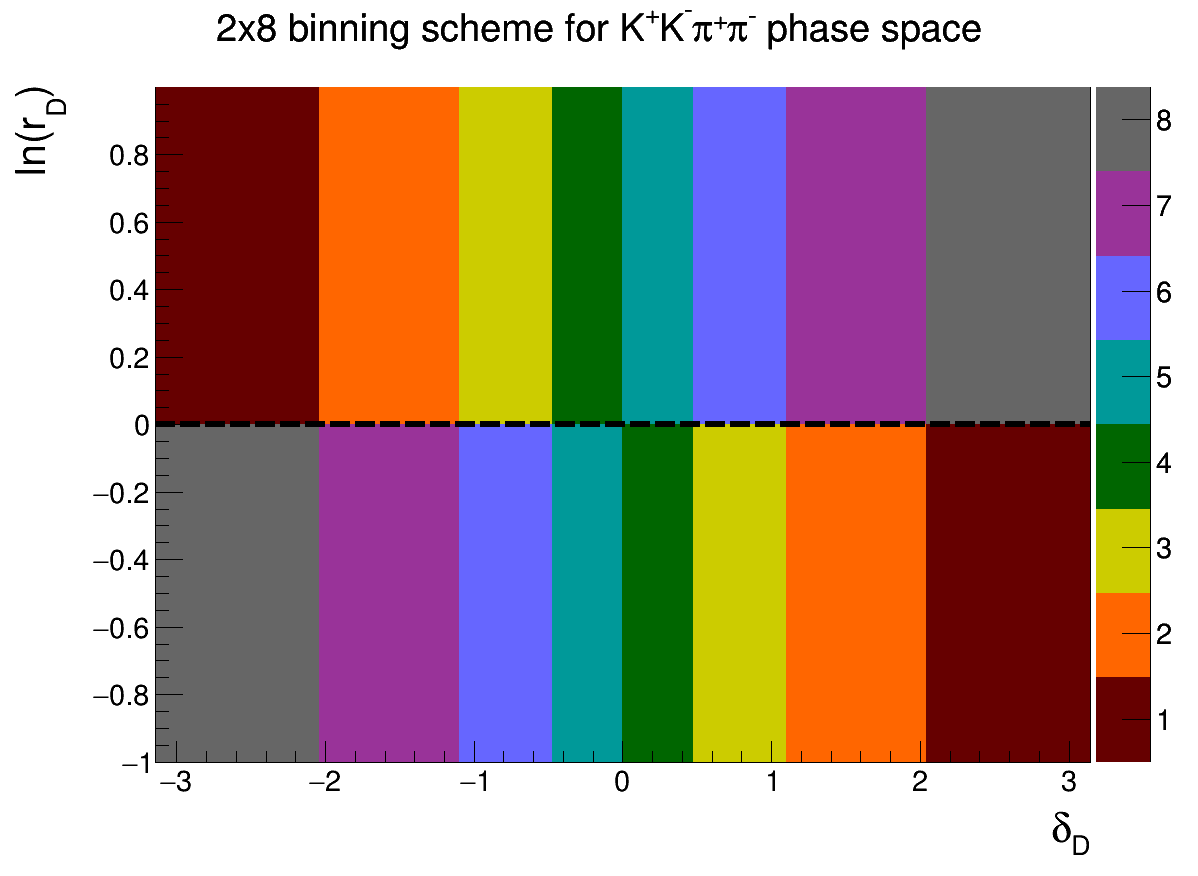
\includegraphics[width=1\textwidth]{Plots/BinningSchemePlot.png}
    \caption{Binning scheme definition for $2\times 8$ bins}
    \label{fig_binning_scheme}
  \end{subfigure}%
  \begin{subfigure}{0.5\textwidth}
    \centering
    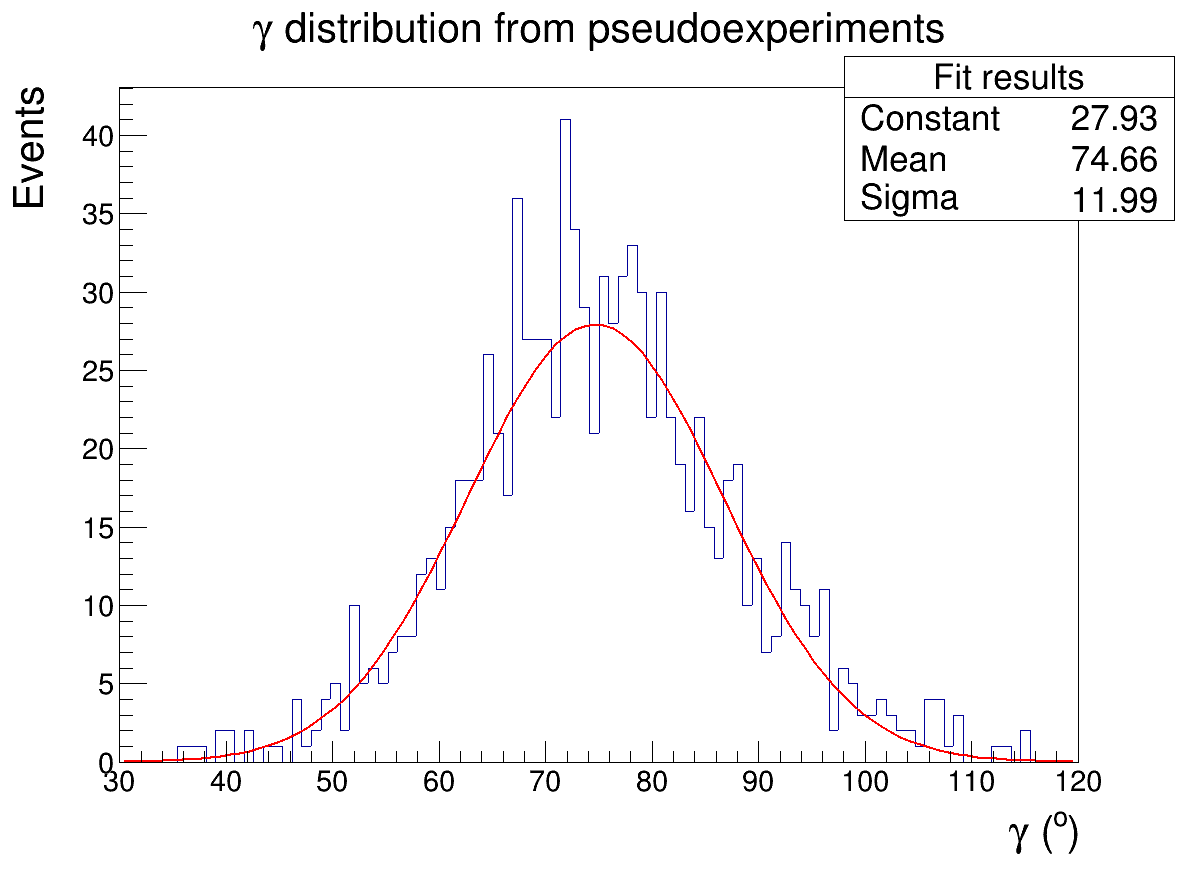
\includegraphics[width=1\textwidth]{Plots/GammaDistribution8BinsVariableWidth.png}
    \caption{Distribution of $\gamma$ from toy study}
    \label{fig_gamma_pull_study}
  \end{subfigure}
  \caption{}
\end{figure}

Fig. \ref{fig_gamma_pull_study} shows the $\gamma$ distribution in the toy experiments. The binned $\gamma$ precision is $\Delta\gamma = \SI{12.0(4)}{\degree}$, which is consistent with the unbinned benchmark and $Q = 0.90$. The pull distributions of $x_\pm^{DK}$, $y_\pm^{DK}$, $\gamma$, $\delta_B$ and $r_B$ have mean and standard deviations consistent with zero and one, respectively, except for $r_B$, which has a small bias.

%%%%%%%%%%%%%%%%%%%%%%%%%%%%%%%%%%%%%%%%%%%%%%%%%%%%%%%%%%%%%%%
\section{\texorpdfstring{$B^\pm$}{B} candidate selection}
\noindent The $B^\pm\to (K^+K^-\pi^+\pi^-)_Dh^\pm$ candidates in the LHCb dataset are reconstructed using standard requirements from Ref. \cite{cite_LHCbGGSZKSpipi}. The $D$ invariant mass must be within $\SI{25}{\mega\eV}$ of the $D^0$ mass. The tracks are refitted with the $D$ invariant mass constrained and its momentum pointing towards $B^\pm$. A cut on $\chi^2$ from this fit removes the $D$ mass sidebands.

$B^\pm\to K^+K^-\pi^+\pi^-h^\pm$ candidates form a charmless background in the $B^\pm$ mass spectrum, but does not peak in the $D$ mass spectrum. To estimate the contamination, the $\chi^2$ cut was removed to preserve the $D$ mass sidebands. Inside the mass region $m(K^+K^-\pi^+\pi^-)\in[1770, 1820]\si{\mega\eV}$, a fit to the $B^\pm$ mass spectrum gives a yield of $\SI{2605(57)}{}$. A flight significance cut, defined as the flight distance divided by its error, reduces this yield to $\SI{110(19)}{}$. No charmless background was found for $B^\pm\to D\pi^\pm$.

A significant mis-ID background is $B^\pm\to Dh^\pm$, $D\to K^\pm\pi^\mp\pi^\pm\pi^\mp$, where a pion is identified as a kaon. A Monte Carlo (MC) simulation sample indicated that $7.2\%$ of $B^\pm$ candidates inside the signal region are $D\to K^\pm\pi^\mp\pi^\pm\pi^\mp$. A tighter particle identification requirement reduces this to $1.8\%$ while keeping $93\%$ of $D\to K^+K^-\pi^+\pi^-$ candidates.

For combinatorial background, a Boosted Decision Tree (BDT) was trained using MC samples as signal and the region $m(Dh^\pm)\in[5800, 7000]\si{\mega\eV}$ in data as background. $99.4\%$ of the combinatorial background was removed and $93.0\%$ of the signal remained.

%%%%%%%%%%%%%%%%%%%%%%%%%%%%%%%%%%%%%%%%%%%%%%%%%%%%%%%%%%%%%%%
\section{\texorpdfstring{$B^\pm$}{B} global mass fit and binned CP fit}
\noindent A global ML fit of the $B^\pm$ mass spectrum, shown in Fig. \ref{fig_Bmass_Global}, was performed to determine global yields and shape parameters, with shape parameterizations from Ref. \cite{cite_LHCbGGSZKSpipi}. The final analysis requires minor adjustments. Currently, only Run $2$ data have been processed.

\begin{figure}[H] 
  \centering
  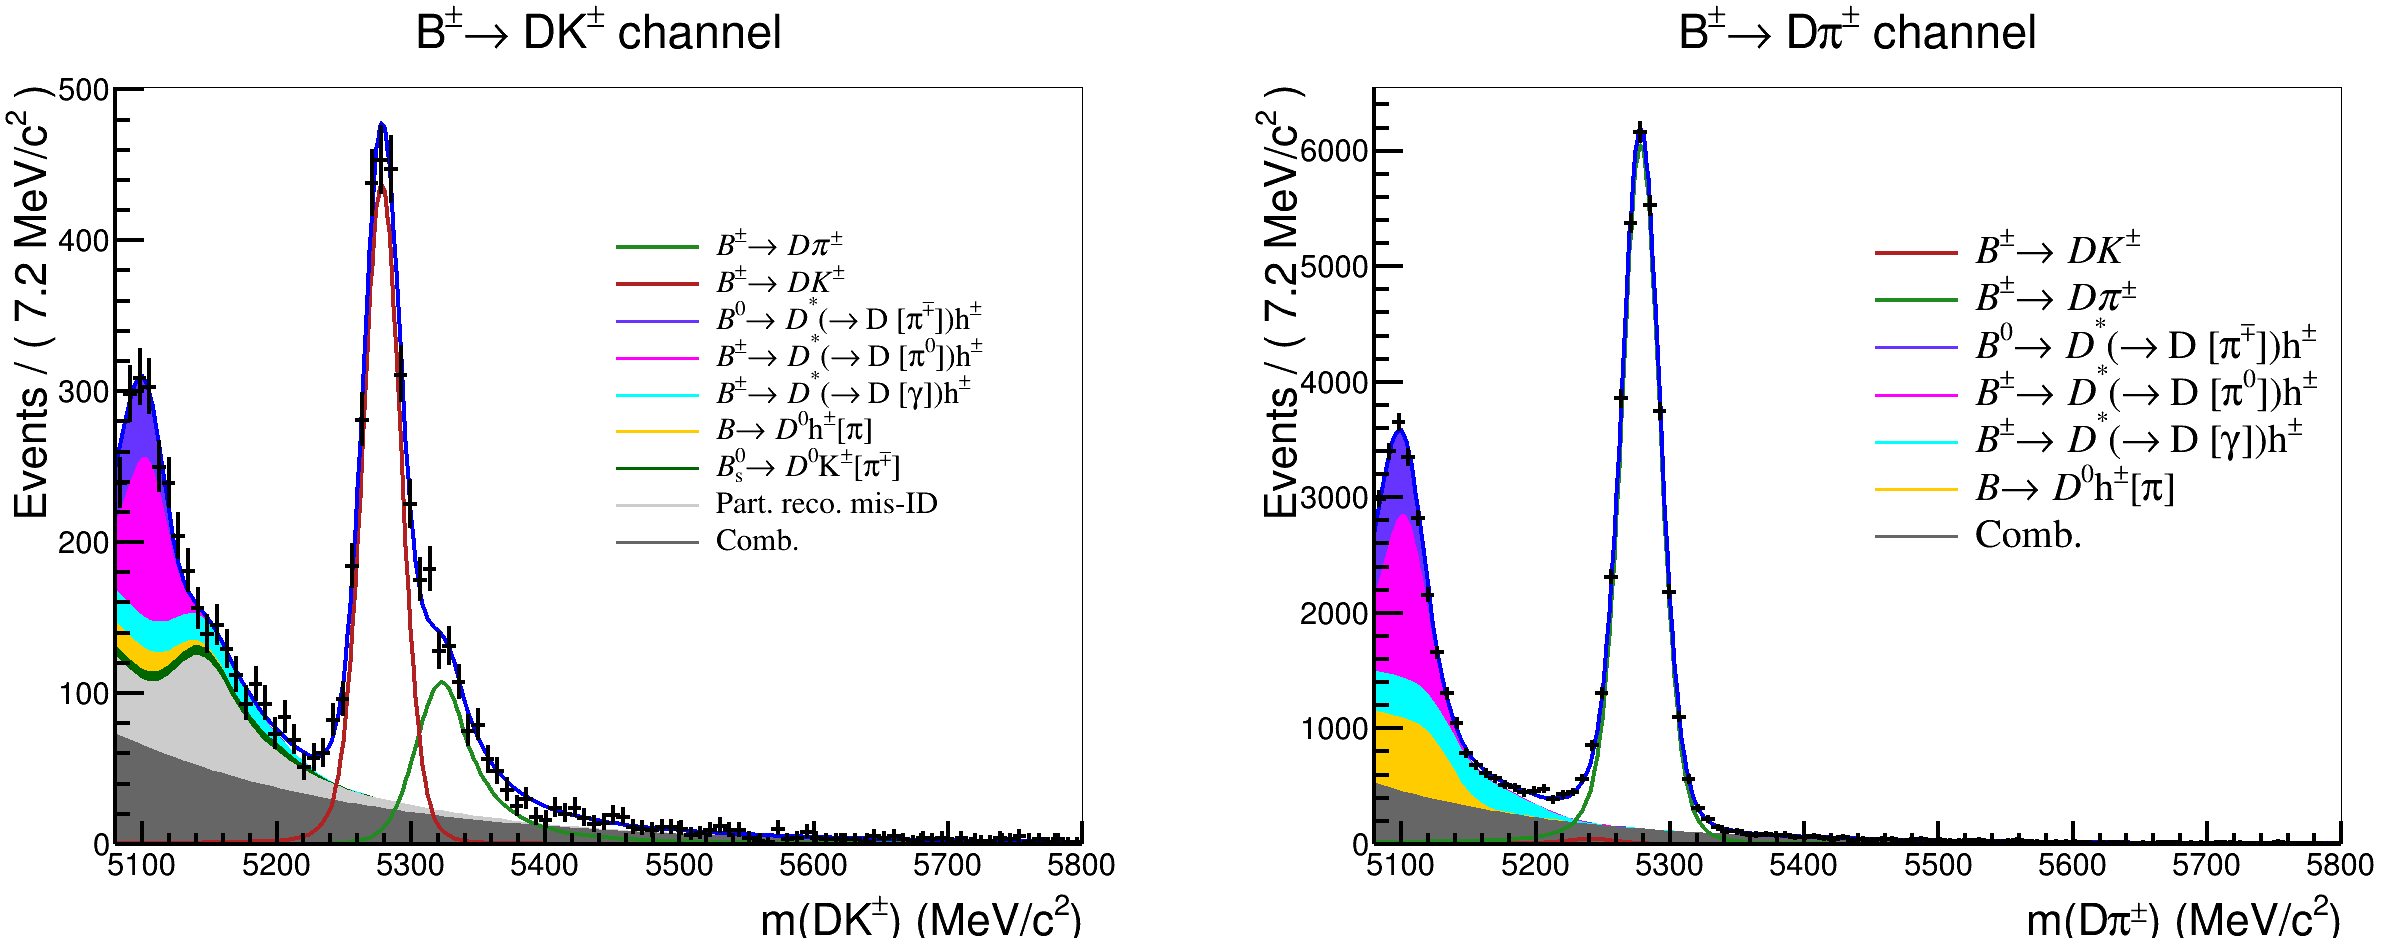
\includegraphics[width=1\textwidth]{Plots/GlobalFit.png}
  \caption{Global mass fit of $B^\pm\to DK^\pm$ (left) and $B^\pm\to D\pi^\pm$ (right) in LHCb data.}
  \label{fig_Bmass_Global}
\end{figure}

The combinatorial background is parameterized by an exponential function. The signal is a sum of a Gaussian $f_\text{G}(m|m_B, \sigma)$ and a modified Gaussian,

\begin{equation}
  f_\text{MG}(m|m_B, \sigma, \alpha_L, \alpha_R, \beta)\propto
  \begin{cases}
    \exp\Big(\frac{-\Delta m^2(1 + \beta\Delta m^2)}{2\sigma^2 + \alpha_L\Delta m^2}\Big), \quad \Delta m = m - m_B < 0 \\
    \exp\Big(\frac{-\Delta m^2(1 + \beta\Delta m^2)}{2\sigma^2 + \alpha_R\Delta m^2}\Big), \quad \Delta m = m - m_B > 0, \\
  \end{cases}
\end{equation}
which accounts for the radiated tail. To the left of the signal are partially reconstructed $B_{(s)}$ decays where a $\pi^\pm$ or $\gamma$ is missed, indicated by $[\pi/\gamma]$. For $B^\pm\to DK^\pm$, there is a mis-ID component of $B^\pm\to D\pi^\pm$ , and a partially reconstructed mis-ID component, where $\pi^\pm$ is misidentified as $K^\pm$. The $B^\pm\to DK^\pm$ signal yield, from Run $2$ alone, is $\SI{2290(59)}{}$, which is higher than the original estimate. The $B^\pm\to D\pi^\pm$ yield is $\SI{33113(211)}{}$.

Finally, $B^\pm$ candidates are split by charge and bins, using the binning in Fig. \ref{fig_binning_scheme}. The current study uses $c_i$ and $s_i$ from the LHCb model. A fit is performed with shape parameters fixed from the global fit, but the yields are floated. Fig. \ref{fig_cp_observables} shows the fitted CP observables. The geometrical angle between $(x_\pm, y_\pm)$ is $2\gamma$, but its exact value is blinded.

To check the fit robustness, $1000$ toy datasets are generated, for both global and CP fits, using the fitted parameters. Each toy is run through the fitting procedure. All CP observables had pulls consistent with zero mean and unit standard deviation.

\begin{figure}[H] 
  \centering
  \begin{subfigure}{0.50\textwidth}
    \centering
    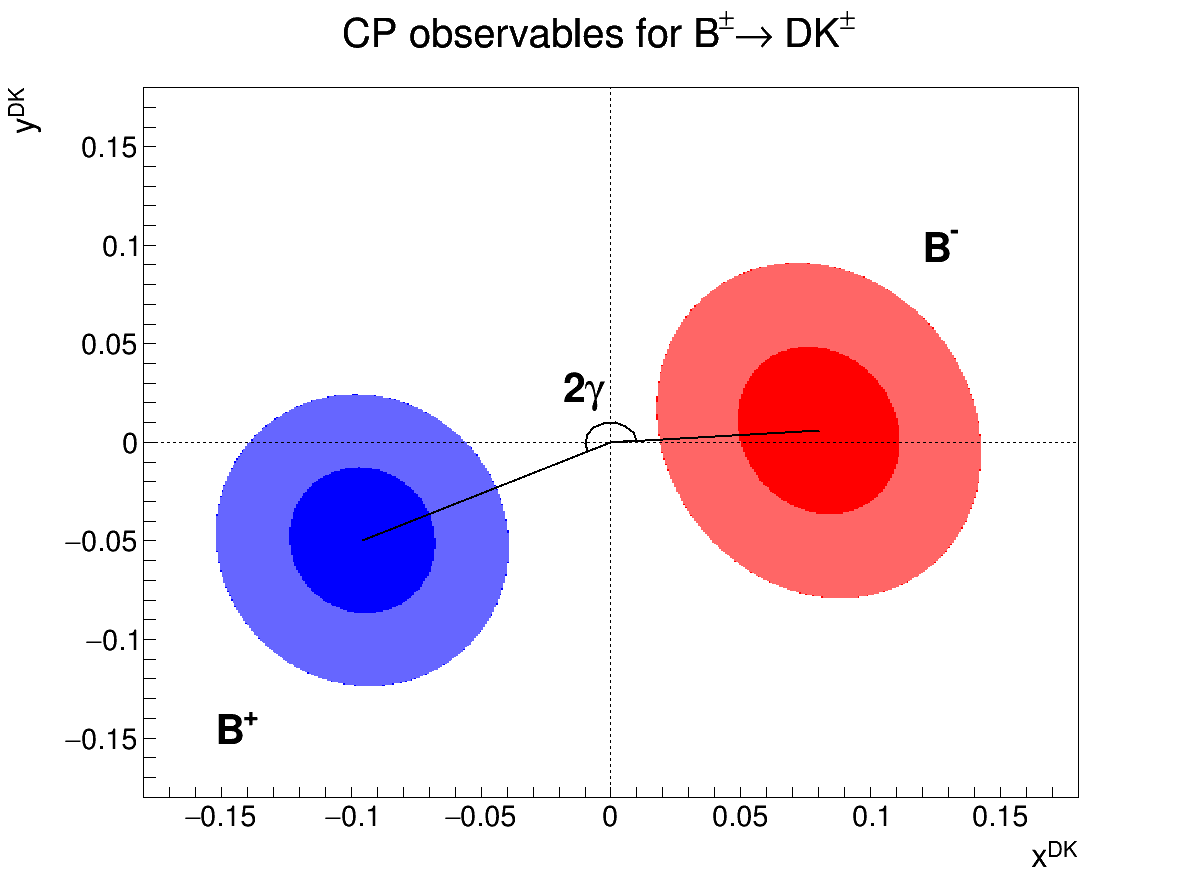
\includegraphics[width=1\textwidth]{Plots/CPContours.png}
  \end{subfigure}%
  \begin{subfigure}{0.50\textwidth}
    \centering
    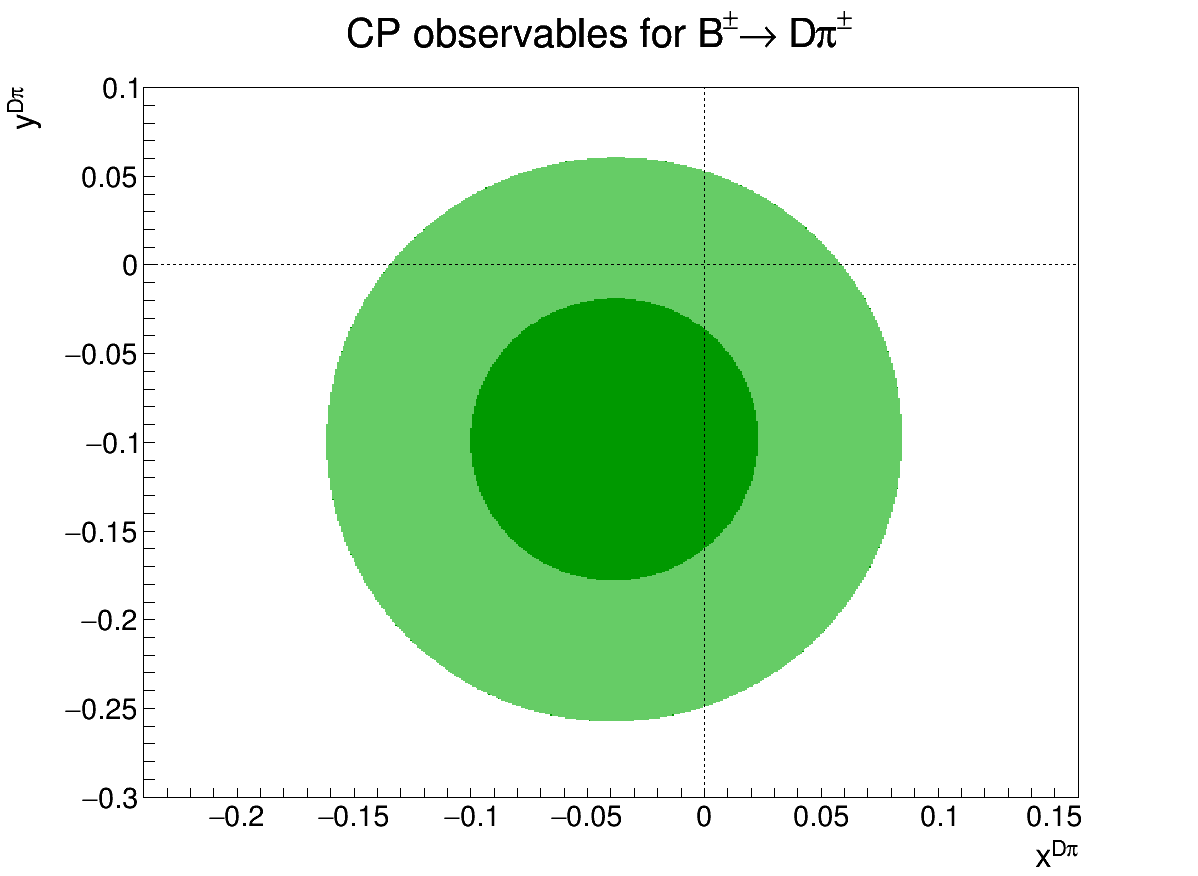
\includegraphics[width=1\textwidth]{Plots/CPXiContours.png}
  \end{subfigure}
  \caption{Confidence levels at $68.2\%$ and $95.5\%$ of $(x_\pm^{DK}, y_\pm^{DK})$ (left) and $(x_\xi^{D\pi}, y_\xi^{D\pi})$ (right).}
  \label{fig_cp_observables}
\end{figure}

%%%%%%%%%%%%%%%%%%%%%%%%%%%%%%%%%%%%%%%%%%%%%%%%%%%%%%%%%%%%%%%
\section{External strong-phase input from BESIII}
\noindent Event reconstruction at BESIII follows Ref. \cite{cite_KSKKAnalysis}. The single tag yield is obtained from a ML fit to the beam constrained $D$ mass $M_\text{BC} = (E_\text{beam}^2 - \abs{\sum_i\vb{p}_i}^2)^{1/2}$, shown in Fig. \ref{fig_styield} for $D\to K^+K^-\pi^+\pi^-$. Peaking backgrounds are accounted for using inclusive MC. The main component, in green, is $D\to K_S^0K^+K^-$. The signal shape is a MC sample convolved with a Gaussian. An Argus shape parameterizes the combinatorial background.

\begin{figure}[H] 
  \centering
  \begin{subfigure}{0.5\textwidth}
    \centering
    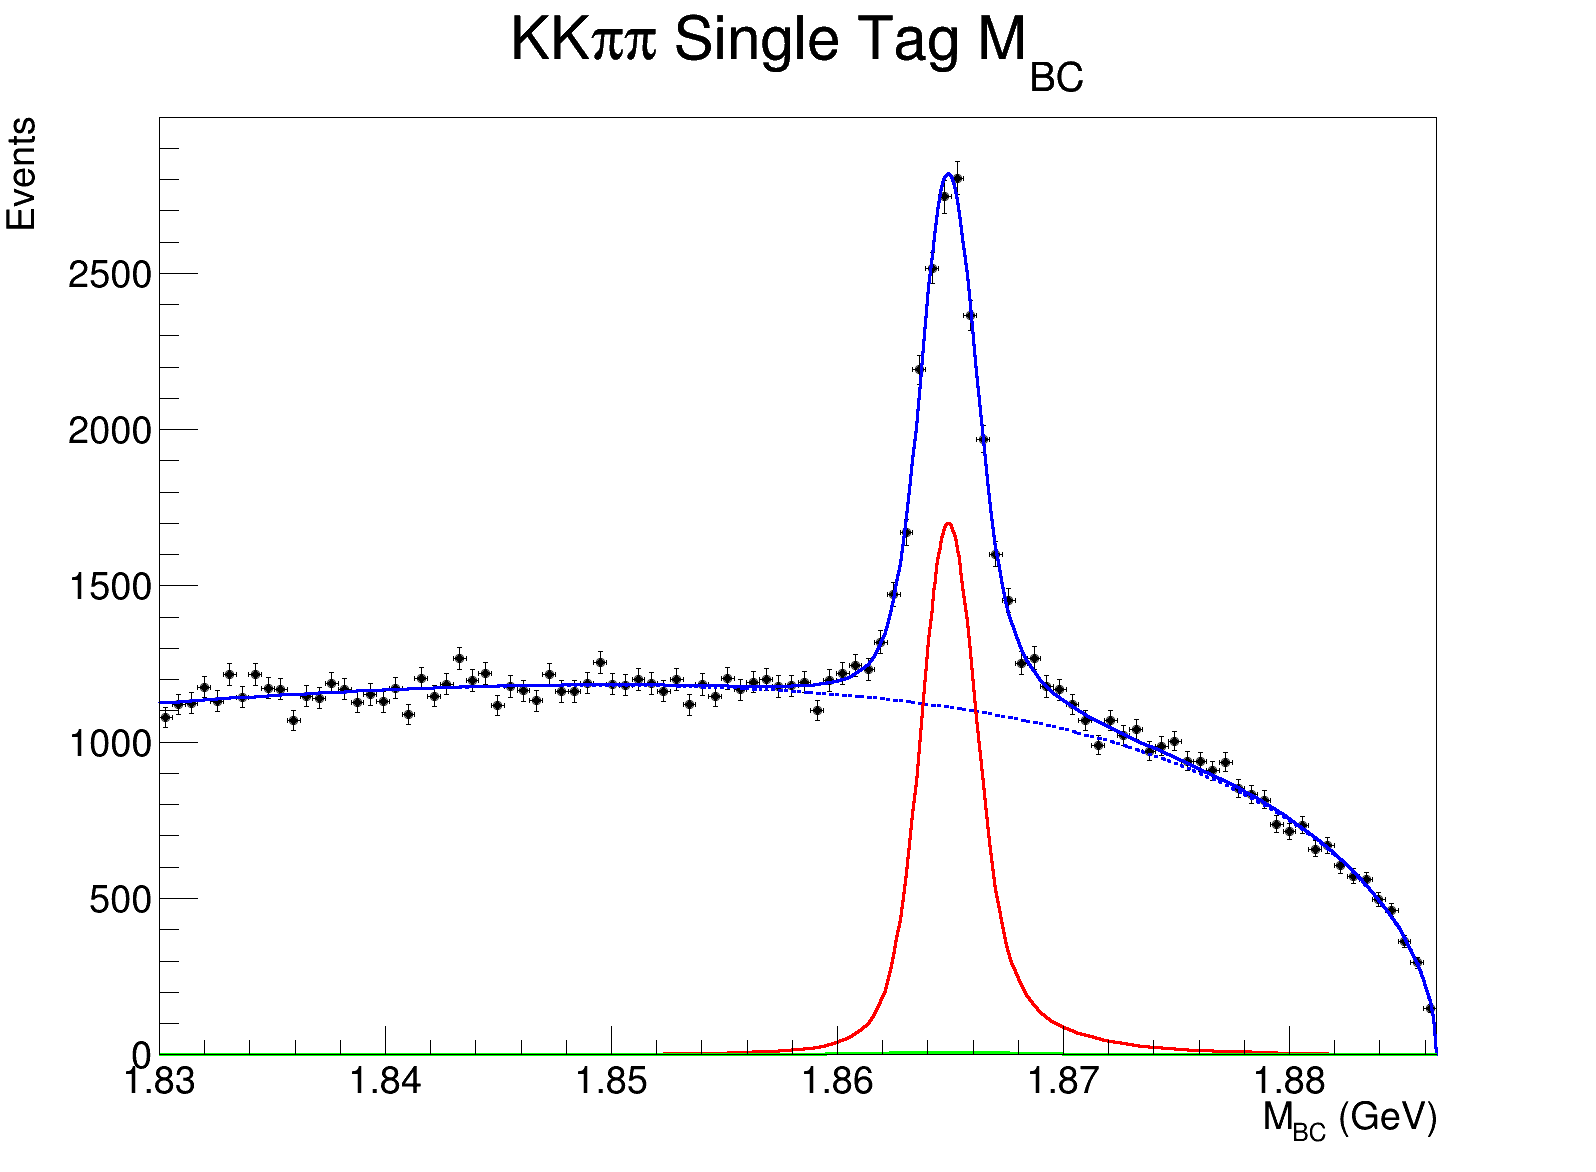
\includegraphics[width=1\textwidth]{Plots/KKpipiSingleTagMBCPlot.png}
    \caption{}
    \label{fig_styield}
  \end{subfigure}%
  \begin{subfigure}{0.5\textwidth}
    \centering
    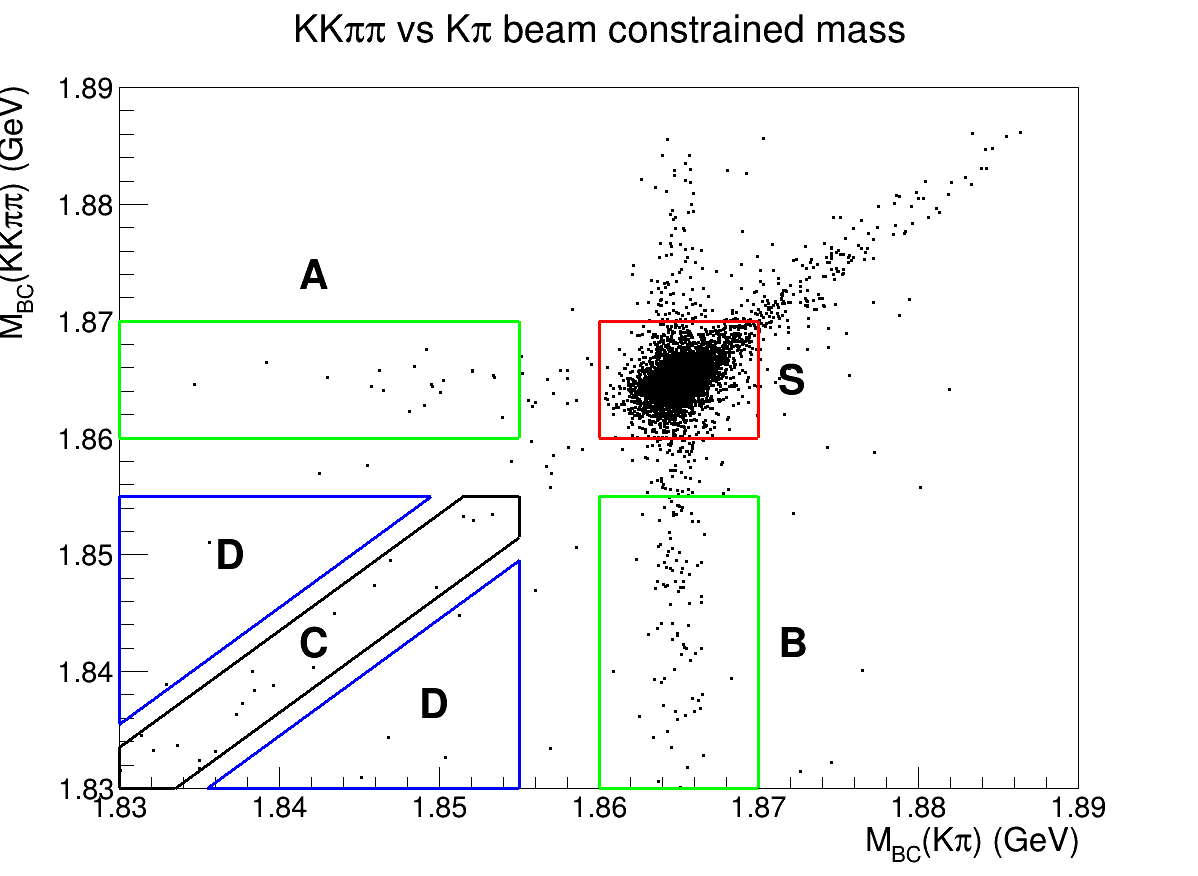
\includegraphics[width=1\textwidth]{Plots/KpiDoubleTagYield.png}
    \caption{}
    \label{fig_dtyield}
  \end{subfigure}
  \caption{$M_\text{BC}$ of single tag $K^+K^-\pi^+\pi^-$ (left) and double tag $K^+K^-\pi^+\pi^-$ vs $K^\mp\pi^\pm$ (right).}
\end{figure}

For double tag yields, a sideband subtraction technique is used. Fig. \ref{fig_dtyield} shows $D\to K^+K^-\pi^+\pi^-$ versus $D\to K^\pm\pi^\mp$ events, where the $M_\text{BC}$ for each $D$ meson is plotted in a $2$D scatter plot. Region $S$ is the signal region, while $A$ and $B$ contain only one real $D$ meson. In region $C$, daughters have been swapped between the $D$ mesons. Region $D$ contains non-charm background. The background is estimated using

\begin{equation*}
  B = P + \frac{a_S}{a_D}Y_D + \sum_{i = A, B, C}\frac{a_S}{a_i}\Big(Y_i - \frac{a_i}{a_D}Y_D\Big),
\end{equation*}
where $P$ is the peaking background, and $Y_i$ and $a_i$ are the yield and area of region $i$. The single and double tag yields are used in a fit of Eqs. \eqref{eq_Mi}-\eqref{eq_Mij} to obtain $c_i$ and $s_i$.

Fig. \ref{fig_cpflavour_yield} shows, on the left, $D\to K^\pm\pi^\mp$ double tag yields with the LHCb model prediction, using $2\times 4$ bins. On the right are the double tag yields with CP odd and even tags $K_S^0\pi^0$ and $K^+K^-$, normalized by $K^\pm\pi^\mp$ yields. The agreement is satisfactory, but the yields are not corrected for efficiencies yet, so perfect agreement is not expected.

\begin{figure}[H] 
  \centering
  \begin{subfigure}{0.5\textwidth}
    \centering
    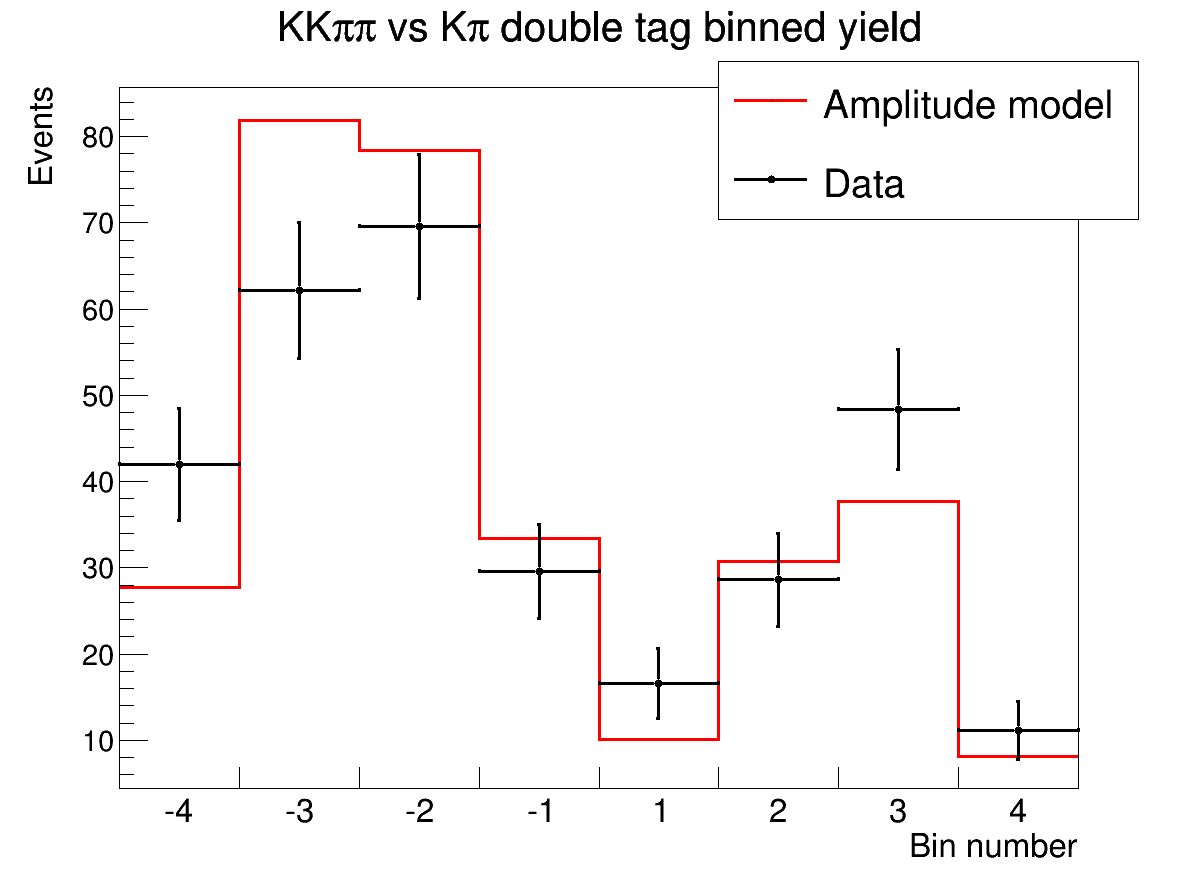
\includegraphics[width=1\textwidth]{Plots/DoubleTagYieldFlavour.png}
  \end{subfigure}%
  \begin{subfigure}{0.5\textwidth}
    \centering
    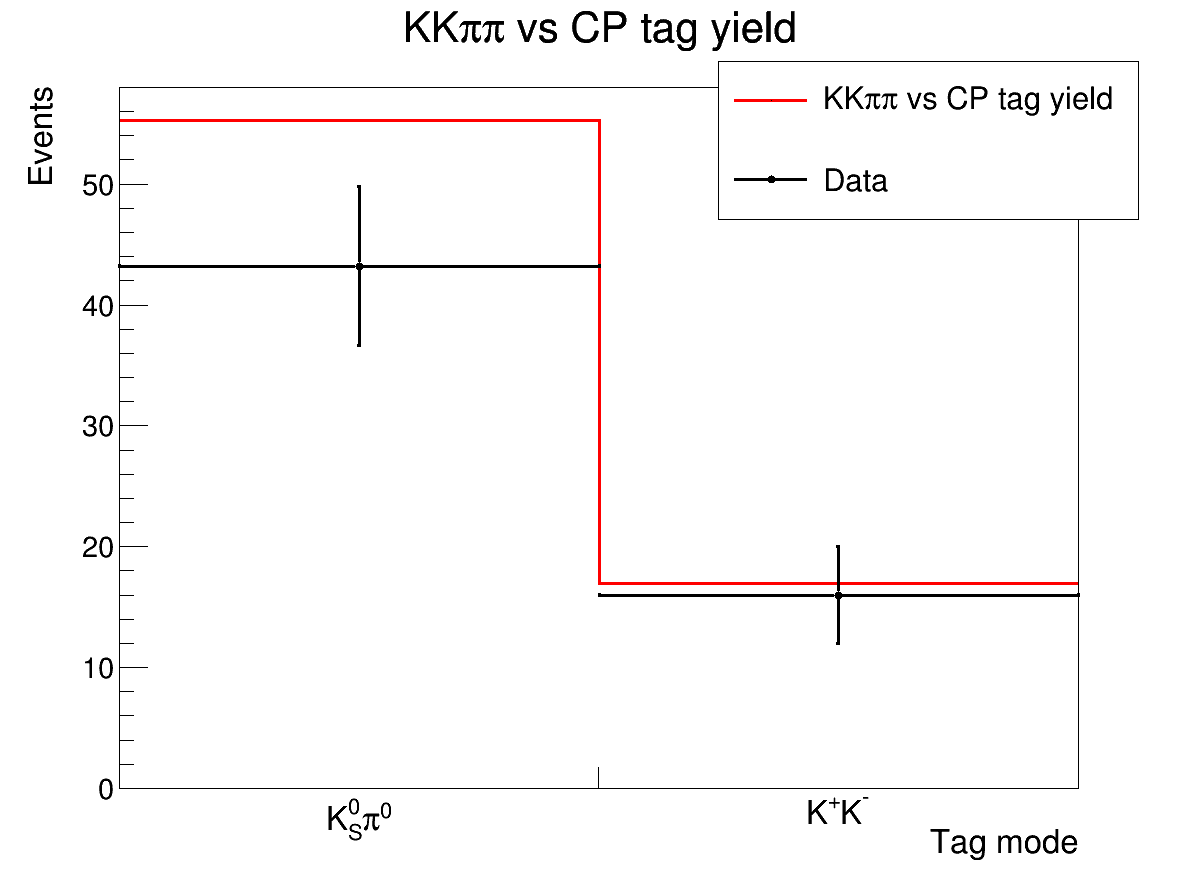
\includegraphics[width=1\textwidth]{Plots/DoubleTagYieldInclusiveCP.png}
  \end{subfigure}
  \caption{Double tag yield of $K^\pm\pi^\mp$ (left), and $K^+K^-$ and $K_S^0\pi^0$ (right).}
  \label{fig_cpflavour_yield}
\end{figure}

%%%%%%%%%%%%%%%%%%%%%%%%%%%%%%%%%%%%%%%%%%%%%%%%%%%%%%%%%%%%%%%
\section{Conclusion and future work}
\noindent The current results at both LHCb and BESIII are consistent with expectations. The next steps in the LHCb analysis are cut optimizations and systematics studies. For BESIII, all tag mode selections must be finalized and the yields determined on the current and future datasets. The analyses will be combined into a first $\gamma$ determination in this channel.

%%%%%%%%%%%%%%%%%%%%%%%%%%%%%%%%%%%%%%%%%%%%%%%%%%%%%%%%%%%%%%%                                                                          
\bibliography{references}
\bibliographystyle{unsrt}

%%%%%%%%%%%%%%%%%%%%%%%%%%%%%%%%%%%%%%%%%%%%%%%%%%%%%%%%%%%%%%%
\newpage
\section*{DPhil thesis plan}
\begin{enumerate}
  \item{Introduction and theory}
  \item{LHCb and BESIII detectors}
  \item{TORCH sub-detector (Time Of internally Reflected CHerenkov light)}
  \item{Formalism and optimization of binning scheme}
  \item{BESIII event selection}
  \item{Determination of strong-phases}
  \item{LHCb candidate selection}
  \item{Global $B^\pm$ mass spectrum fit}
  \item{Binned CP fit and determination of $\gamma$}
  \item{Conclusion}
\end{enumerate}

\end{document}